% Chapter 3

\chapter{DESIGN AND ARCHITECTURE}

% \begin{figure}[hbt] 
% \begin{center}
% \includegraphics[scale=.40]{./figures/bddig1}
% \caption{\label{fig:BDDD}A BDD where some boolean variables occur more than
% once on an evaluation path.}
% \end{center}
% \end{figure}

We propose a design quality assessment system based on Machine
learning models that utilize an abstract syntax tree (AST) to
represent programs. The ML models are regression models that are
trained on assessed student programs to predict a score between zero
and one. Each feature used by a model is designed to be meaningful to
human interpretation and is based on statistics collected from the
program's AST. We intentionally do not use deep learning as it would
make the representation of the program difficult to
understand. Personalized feedback is generated based on each feature
of an individual program. By swapping a feature's value for an
individual program with the average feature value of good programs, it
is possible to determine which changes need to be made to the program
to improve design


\section{TRAINING} 

The dataset contains the code and corresponding scores for each of the
student programs. Features from code were extracted by using two
ways. Some features were extracted directly from the code. For the
other features, the code was first transformed into an Abstract Syntax
Tree(AST); then the features were extracted from the AST. The extracted
features were used to train the model. Three models were trained
separately: Support vector regressor, Random forest and Multi layer
perceptron. The models trained were all regression models which were
trained to predict the scores that should be given to the evaluated
codes.

\begin{figure}[h]
\centering
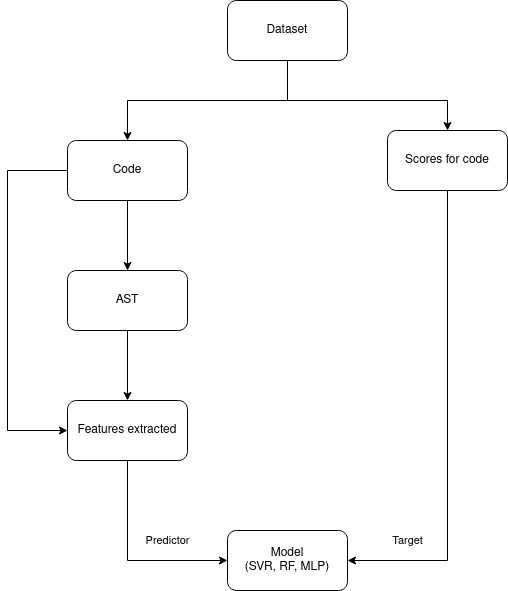
\includegraphics[width=0.9\textwidth]{./training.jpg}
\caption{Training}
\label{fig1}
\end{figure}

\newpage

\section{DEPLOYMENT} 

The student code is the input. Features are extracted from the code as
explained in the section above. Some features are extracted from the
code itself and the rest from an AST representation of the code. This
feature set is input into the trained models from the previous
section. The model predicts a score for the input code based on the
feature set.

In order to avoid the need for a dataset with explicit feedback
annotation, we use our model, trained on predicting design score, to
evaluate how changes in program features would lead to a higher
assessed score. Using the training data, we compute an average feature
vector $x$ of all the ``good'' programs. To generate feedback for a
program, its feature vector is compared to the average.

\begin{figure}[h]
\centering
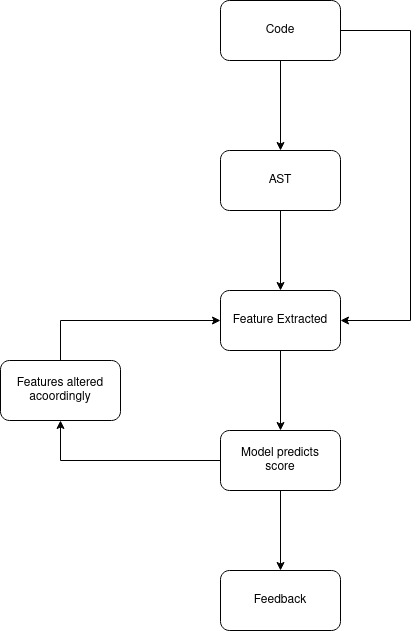
\includegraphics[scale=0.7]{./Deployment.jpg}
\caption{Deployment}
\label{fig1}
\end{figure}

\section{ALGORITHMS}

After representing code solutions as feature vectors, the dataset was
exported to perform training for machine learning models. The
following models
\begin{itemize}
    \item Support Vector Machine (SVM)
    \item Random Forest 
    \item Multi Layer Perceptron (MLP)
\end{itemize}
were employed for training. The detailed description of the mentioned
algorithms are listed below.

\section{SUPPORT VECTOR MACHINE}

In machine learning, Support Vector Machines are supervised learning
models with associated learning algorithms that analyze data used for
classification and regression. Support Vector Regression \cite{D} is a
supervised learning algorithm that is used to predict continuous
values. Support Vector Regression uses the same principle as the
Support Vector Machine (SVM). The objective of a support vector
machine algorithm is to find a hyperplane in an n-dimensional space
that distinctly classifies the data points. The data points on either
side of the hyperplane that are closest to the hyperplane are called
Support Vectors. These influence the position and orientation of the
hyperplane and thus help build the SVM.

\subsection{Hyperparameters in SVR}

Following are the various key hyper parameters used in Support Vector Regression.
\begin{figure}[h]
\centering
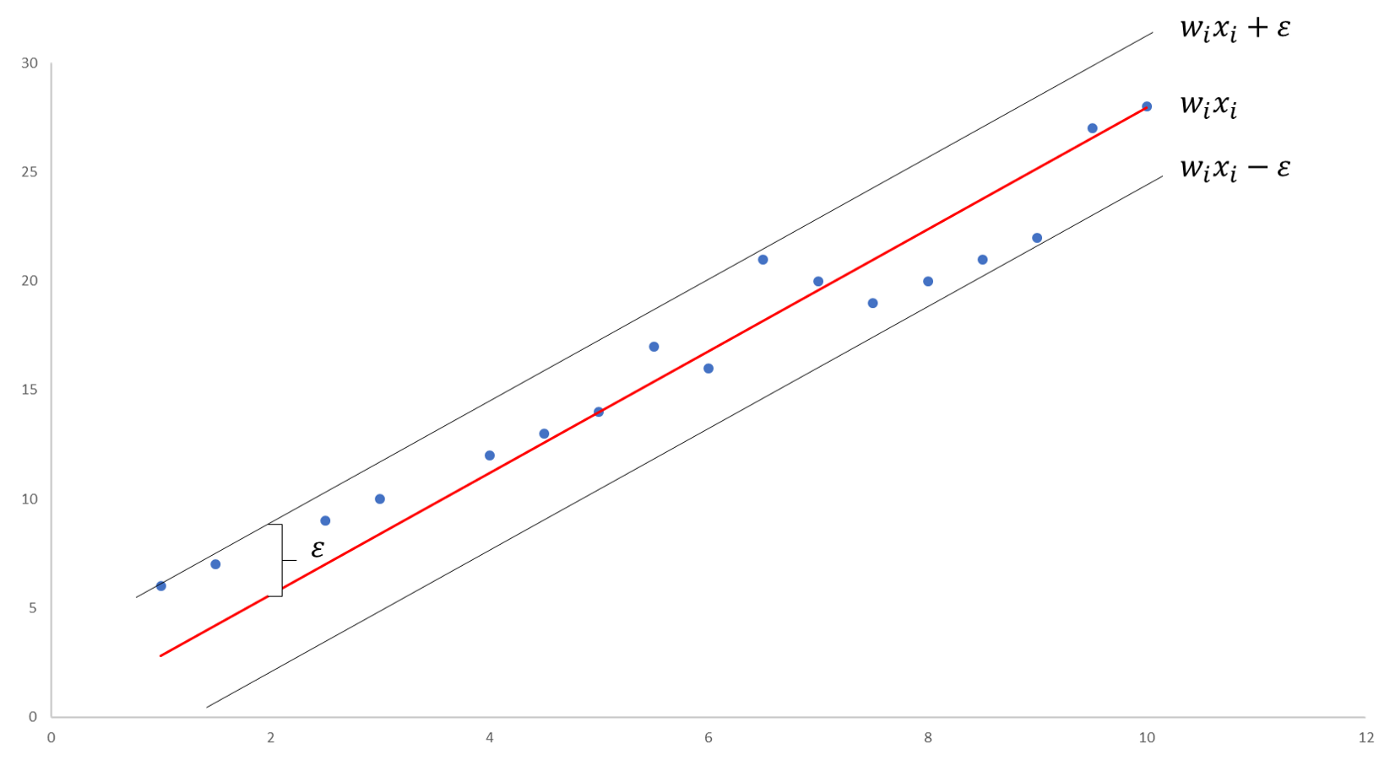
\includegraphics[width=1\textwidth, height=15cm]{./figures/svm.png}
\caption{Simple SVR}
\label{fig1}
\end{figure}

\begin{itemize}
\item \textbf{Hyperplane} (Red line in Figure~6.1) \\ Hyperplane is a
  decision boundary that is used to predict the continuous output. The
  data points on either side of the hyperplane that are closest to the
  hyperplane are called Support Vectors. These are used to plot the
  required line that shows the predicted output of the algorithm.
\item \textbf{Kernel} \\ A kernel is a set of mathematical functions
  that takes data as input and transform it into the required
  form. These are generally used for finding a hyperplane in the
  higher dimensional space.
\item \textbf{Boundary Lines} (Grey lines in Figure~6.1) \\ These are
  the two lines that are drawn around the hyperplane at a distance of
  \textbf{$\epsilon$} (epsilon). It is used to create a margin between
  the data points.
\end{itemize}

\subsection{Support Vector Regression}

Support Vector Regression (SVR) finds the best fit line or the
hyperplane that has the maximum number of points. Unlike other
regression models that try to minimize the error between the real and
predicted value, the SVR tries to fit the best line within a threshold
value (the distance between the hyperplane and boundary line).  Hence,
we are going to take only those points that are within the decision
boundary and have the least error rate, or are within the margin of
tolerance. This gives us a better fitting model.

%\newpage

\section{RANDOM FOREST}

Random forest is a supervised machine learning algorithm that is used
widely in classification and regression problems. The functioning of
Random Forest is contingent on three main factors,
\begin{itemize}
\item Decision Trees
\item Ensemble Learning
\item Bootstrapping
\end{itemize}

The following subsections % (6.2.1, 6.2.2 and 6.2.3)
detail on the mentioned factors description.

\subsection{Ensemble Learning}

Ensemble learning is the process of using multiple models, trained
over the same data, averaging the results of each model, ultimately
finding a more accurate predictive/classification result. The
requirement for ensemble learning is that the errors of each model (in
this case decision tree) are independent and different from tree to
tree.

\subsection{Decision Tree}

\begin{figure}[h]
\centering
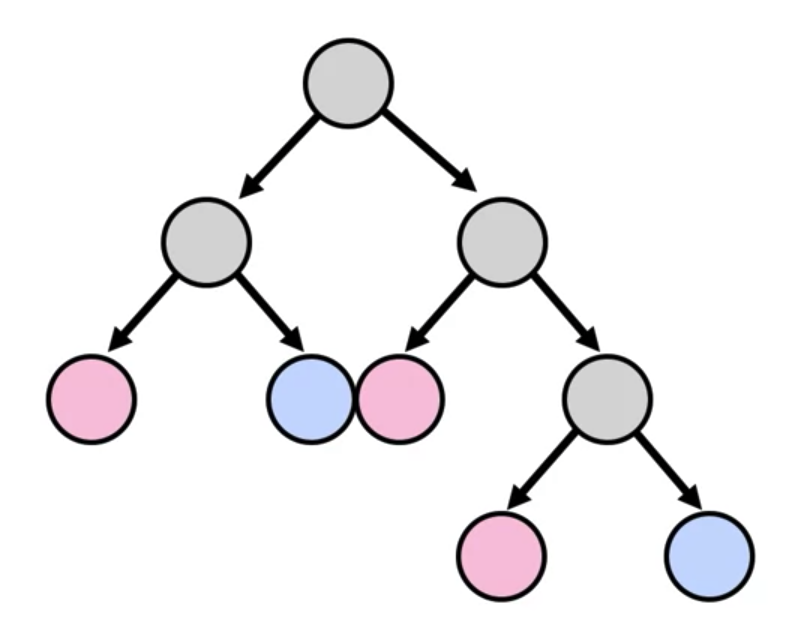
\includegraphics[scale=.5]{./figures/dectree.png}
\caption{Decision tree layout}
\label{fig1}
\end{figure}

Decision Trees are used for both regression and classification
problems. The goal is to create a model that predicts the value of a
target variable by learning simple decision rules inferred from the
data features. They start with the root of the tree and follow splits
based on variable outcomes until a leaf node is reached and the result
is given. Figure~6.2 details a visual representation of the decision
tree layout.

\subsection{Bootstrapping}

Bootstrapping is the process of randomly sampling subsets of a dataset
over a given number of iterations and a given number of
variables. These results are then averaged together to obtain a more
accurate result.

\subsection{Random Forest Regression}

\begin{figure}[h]
\centering
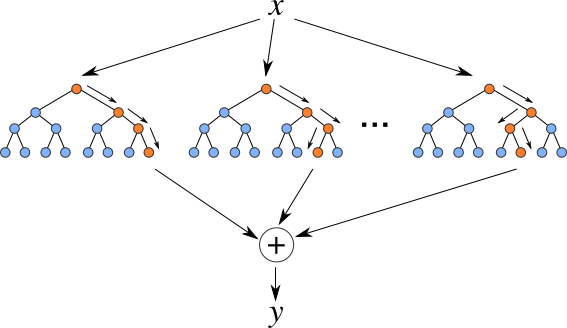
\includegraphics[width=1\textwidth, height=12cm]{./figures/rf.png}
\caption{Simple RF}
\label{fig1}
\end{figure}

The bootstrapping Random Forest algorithm \cite{B} combines ensemble
learning methods with the decision tree framework to create multiple
randomly drawn decision trees from the data, averaging the results to
output a new result that often leads to strong
predictions/classifications. Figure~6.2 documents a visual
representation of random forest wherein $X$ is the feature
vector and $y$ is the target vector.

\section{MULTI LAYER PERCEPTRON}

The Multi Layer Perceptron bases its fundamental design to the
interlinking of several neuron-like structures representing a Neural
Network (NN) architecture. Given $i = 0,1,\ldots,n$ where $n$ is the
number of inputs, the quantities $w_{i}$ are the weights of the
neuron. The inputs $x_{i}$ correspond to features or variables and the
output $y$ to their prediction/estimation. Figure~6.4 shows the
simplified representation of the above steps.

\begin{figure}[h]
\centering
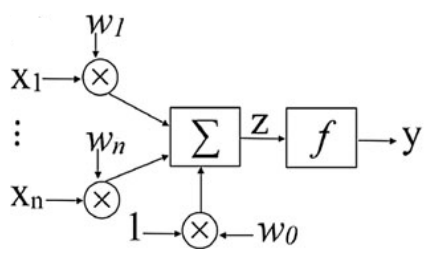
\includegraphics[]{./figures/perceptron.png}
\caption{Perceptron model}
\label{fig1}
\end{figure}

The weighting step involves the multiplication of each input feature
value by its weight ${w_ix_i}$ and in the second step they are added
together $(x_{0}w_{0} + x_{1}w_{1} + ... + x_{n}w_{n})$. The third is
the transfer step where an activation function f (also called a
transfer function) is applied to the sum producing an output $y$
presented as
\begin{align*}
  z & = \sum_{i=0}^{n} w_{i}x_{i}\\
  y & = f(z)
\end{align*}
wherein $x_{0} = 0$, $w_{0}$ is the bias and $y$ is the output. The
activation function can be of the form of Unit step, Linear or
Logistic operation.

A perceptron can only learn linearly separable functions. For $n$
dimensions, the function is a hyperplane with equation:
\begin{equation}
    \sum_{i=0}^{n} w_{i}x_{i} = 0
\end{equation}

The motive of learning is to optimize the weights by minimizing a cost
function, which is usually a square error between the known vector and
the estimated vector. Optimization techniques such as gradient descent
algorithm can be used to determine the optimum weight
vector. Ultimately, the algorithm converges to a solution reaching an
operational configuration network. However, the perceptron and the
single layer perceptron do not resolve the nonlinearly separable
problem.

\begin{figure}[h]
\centering
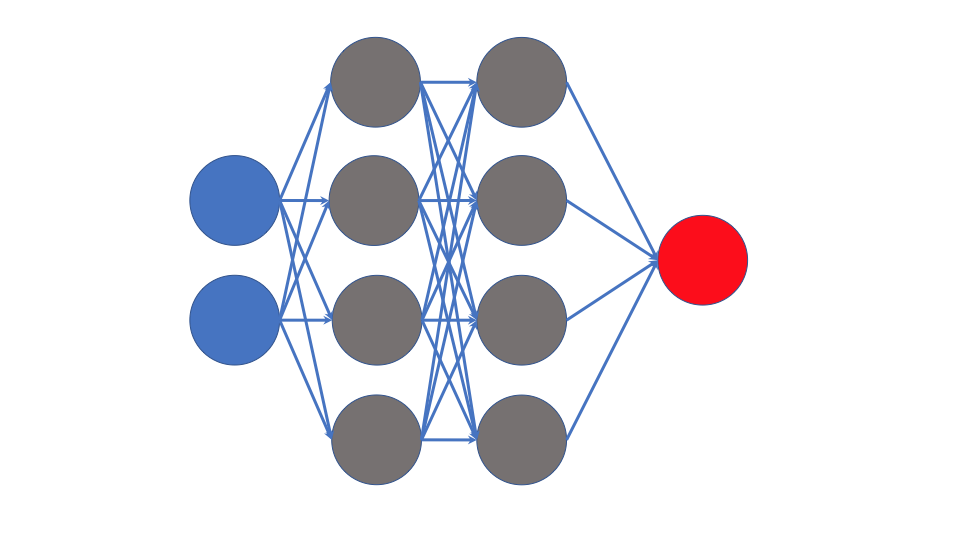
\includegraphics[width=1\textwidth]{./figures/mlp2.png}
\caption{MLP model}
\label{fig1}
\end{figure}

To solve this problem, Multi Layer Perceptron (MLP) architecture is
created by aggregating layers of perceptrons wherein the output of one
layer acts as the input of another layer. Multi Layer Perceptron
\cite{C} is a feedforward neural network that consists of three
layers, the input layer, the hidden layer and the output
layer. Figure~6.5 presents an MLP with two inputs (blue), two hidden
layers (grey) and one output (red).

The input layer receives the input signal to be processed. The
required task such as prediction and classification is performed by
the output layer. An arbitrary number of hidden layers that are placed
in between the input and output layer are the true computational
engine of the MLP. Similar to a feed forward network in a MLP the data
flows in the forward direction from input to output layer. The neurons
in the MLP are trained with the back propagation learning algorithm,
where the weights can be corrected by propagating the errors from
layer to layer starting with the output layer and working
backwards. MLPs are designed to approximate any continuous function
and can solve problems which are not linearly separable.
